\documentclass[12pt,a4paper]{article}
\usepackage{t1enc}
\usepackage{amsmath}
\usepackage{listings}
\usepackage{color}
\usepackage{graphicx}
\usepackage{float}
\usepackage{hyperref}
\usepackage[hungarian]{babel}
\definecolor{mygreen}{rgb}{0,0.6,0}
\definecolor{mygray}{rgb}{0.5,0.5,0.5}
\definecolor{mymauve}{rgb}{0.58,0,0.82}
\setcounter{secnumdepth}{2}

\lstset{
    backgroundcolor=\color{white},
    basicstyle=\footnotesize,
    breakatwhitespace=false,
    breaklines=true,
    captionpos=b,
    commentstyle=\color{mygreen},
    escapeinside={\%*}{*)},
    extendedchars=true,
    frame=single,
    keepspaces=true,
    keywordstyle=\color{blue},
    language=Matlab,
    numbers=left,
    numbersep=5pt,
    numberstyle=\tiny\color{mygray},
    rulecolor=\color{black},
    showspaces=false,
    showstringspaces=false,
    showtabs=false,
    stepnumber=1,
    stringstyle=\color{mymauve},
    tabsize=2,
    title=\lstname
}

\hypersetup{
    colorlinks=true,
    linkcolor=black,
    citecolor=black,
    filecolor=black,
    urlcolor=black,
    pdfborder={0 0 0}
}

\begin{document}

% Cover Page
\begin{titlepage}
    \centering
    \vspace*{\fill}
    \textbf{\Huge Problem 8. - N elemű lánckapcsolás}\\[2cm]
    
\includegraphics[width=0.65\textwidth]{figures/bme_logo_nagy_bordo.jpg}\\[1cm]
    \textbf{\Large Budapest Műszaki és Gazdaságtudományi Egyetem}\\[0.25cm]
    \Large Természettudományi Kar\\[0.25cm]
    \Large Fizika Tanszék\\[2cm]
    \Large Házi feladat\\[0.25cm]
    \Large Műszaki és fizikai problémák számítógépes megoldása (BMETE11AF41 2024/25/1)\\[2cm]
    \Large \textbf{\textit{Szerző:}}\\[0.25cm]
    \Large Kovács Levente (F5UHYT)\\[1cm]
    \Large \today
    \vspace*{\fill}
\end{titlepage}
\newpage

% Page numbering
\pagenumbering{arabic}
% Table of Contents
\tableofcontents
\newpage

\section*{MATLAB Szkript Leírása}

Ez a MATLAB szkript egy RLC létra hálózat viselkedését szimulálja az idő függvényében. A felhasználótól különböző paraméterek megadását kéri a szimulációhoz, beleértve az induktanciát (L), kapacitást (C), forrás belső ellenállását (R0), forrás feszültség amplitúdóját (U0), a létra lépések számát (n) és a szimuláció végidejét (tmax).

\subsection*{A Szkript Által Végrehajtott Lépések}

\begin{enumerate}
    \item A felhasználótól kéri a paraméterek megadását és érvényesíti azokat.
    \item Kiszámítja a lezáró ellenállást (Rt) és beállítja a szimuláció időtartamát.
    \item Inicializálja az állapotváltozókat (az induktorokon átfolyó áramok és a kondenzátorokon lévő feszültségek).
    \item Az \texttt{ode45} megoldót használja a RLC létra hálózatot leíró differenciálegyenletek numerikus megoldására.
    \item Ábrázolja az első, középső és utolsó kondenzátorokon lévő feszültségeket.
    \item Ábrázolja az első, középső és utolsó tekercseken átfolyó áramokat.
    \item Lehetőséget biztosít a felhasználónak további áramok vagy feszültségek ábrázolására specifikus tekercseken vagy kondenzátorokon.
\end{enumerate}

A differenciálegyenleteket az \texttt{odefun} függvény definiálja, amely kiszámítja az állapotváltozók deriváltjait az aktuális állapot és a bemeneti paraméterek alapján.

\subsection*{Paraméterek}

\begin{itemize}
    \item \textbf{L}: Induktancia Henry-ben (H)
    \item \textbf{C}: Kapacitás Farad-ban (F)
    \item \textbf{R0}: Forrás belső ellenállása Ohm-ban (\(\Omega\))
    \item \textbf{U0}: Forrás feszültség amplitúdója Volt-ban (V)
    \item \textbf{n}: Létra lépések száma (pozitív egész szám)
    \item \textbf{tmax}: A szimuláció végideje másodpercben (s)
\end{itemize}

\subsection*{Függvények}

\begin{itemize}
    \item \texttt{odefun}: Meghatározza a RLC létra hálózat differenciálegyenleteit.
\end{itemize}

\subsection*{Kimenetek}

\begin{itemize}
    \item Az első, középső és utolsó kondenzátorokon lévő feszültségek ábrái.
    \item Az első, középső és utolsó induktorokon átfolyó áramok ábrái.
    \item Opcionális ábrák specifikus induktorokon vagy kondenzátorokon lévő áramokról vagy feszültségekről a felhasználó kérésére.
\end{itemize}

\subsection*{MATLAB Kód}
\subsection*{Paraméterek Bekérése és Érvényesítése}

A paraméterek és azok érvényes tartományai a következők:

\begin{itemize}
    \item \textbf{L (Induktivitás)}: Pozitív valós szám, amely az induktanciát Henry-ben (H) adja meg.
    \item \textbf{C (Kapacitás)}: Pozitív valós szám, amely a kapacitást Farad-ban (F) adja meg.
    \item \textbf{R0 (Forrás Belső Ellenállása)}: Pozitív valós szám, amely a forrás belső ellenállását Ohm-ban adja meg.
    \item \textbf{U0 (Forrás Feszültség Amplitúdója)}: Valós szám, amely a forrás feszültség amplitúdóját Volt-ban (V) adja meg.
    \item \textbf{n (Létra Lépések Száma)}: Pozitív egész szám, amely a létra hálózat lépéseinek számát adja meg.
    \item \textbf{tmax (Szimuláció Végideje)}: Nem negatív valós szám, amely a szimuláció végidejét másodpercben (s) adja meg. Ha 0-ra van állítva, a végidő automatikusan kiszámításra kerül a többi paraméter alapján.
\end{itemize}

\subsection*{Lezáró Ellenállás és Szimuláció Időtartama}

A lezáró ellenállást értéke a feladatleírás szerint 
\( R_t = 2 \sqrt{\frac{L}{C}} \)
.

A szimuláció végidejét a felhasználó által megadott érték alapján állítjuk be. Ha a felhasználó 0-t ad meg, akkor a végidő automatikusan kiszámításra kerül a következő képlet alapján:
\[ t_{\text{max}} = 3 \cdot n \cdot \sqrt{L \cdot C} \]

\begin{lstlisting}
    % Lezaro ellenallas kiszamitasa
    Rt = 2 * sqrt(L / C); % Lezaro ellenallas [Ohm]

    % Szimulacio idotartamanak beallitasa
    tspan = [0 tmax];
\end{lstlisting}

\subsection*{Állapotváltozók Inicializálása}

Az állapotváltozókat (az tekercsen átfolyó áramok és a kondenzátorokon lévő feszültségek) inicializáljuk:

\begin{lstlisting}
% Kezdoallapot: minden aram es feszultseg nulla
y0 = zeros(2 * n, 1);
\end{lstlisting}

\subsection*{Differenciálegyenletek Meghatározása}

Az \textbf{odefun} segédfüggvény a differenciálegyenletek meghatározását végzi. Ez a függvény adja vissza az állapotváltozók deriváltjaira rendezett egyenletrendszer jobb oldalát.

\subsubsection{Állapotváltozók definiálása}

A tekercsek áramai (iL) és a kondenzátorok feszültségei (uC) az állapotváltozók, amelyeket a bemeneti vektor (y) alapján határozunk meg.

\begin{lstlisting}
    iL = y(1:n); % Tekercsek aramai
    uC = y(n+1:end); % Kondenzatorok feszultsegei
\end{lstlisting}

\subsubsection{Forrás feszültségének meghatározása}
A forrás feszültsége (Us) az idő (t) függvényében változik. Ha t >= 0, akkor Us = U0, különben Us = 0.

\begin{lstlisting}
    if t >= 0
        Us = U0;
    else
        Us = 0;
    end
\end{lstlisting}

\subsubsection{Differenciálegyenletek felírása}
\[
\begin{aligned}
    i_C &= C \frac{du_C}{dt} \\
    u_L &= L \frac{di_L}{dt}
\end{aligned}
\]
\begin{lstlisting}
    diL_dt = zeros(n, 1);
    duC_dt = zeros(n, 1);
\end{lstlisting}

\pagebreak

\subsubsection{Egyenletek felírása minden létrafokra}
Egy \textbf{for} ciklus segítségével minden létrafokra felírjuk az egyenleteket. A végén visszaadjuk az \textbf{ÁVLNA} egyenleteit egy vektorban.

\begin{lstlisting}
    for i = 1:n
        if i == 1
            U_be = Us - R0 * iL(i); % Elso letrafok bemeneti feszultsege
        else
            U_be = uC(i-1); % Elozo kondenzator feszultsege
        end
        
        if i == n
            I_ki = uC(i) / Rt; % Lezaro ellenallas a vegen
        else
            I_ki = iL(i+1); % Kovetkezo tekercs arama
        end
        
        % Tekercs karakterisztikaja
        diL_dt(i) = (U_be - uC(i)) / L;
        
        % Kondenzator karakterisztikaja
        duC_dt(i) = (iL(i) - I_ki) / C;
    end

    % Kombinalt eredmeny
    dydt = [diL_dt; duC_dt];
\end{lstlisting}

\subsection*{Differenciálegyenletek Megoldása}

Az \texttt{ode45} megoldót használjuk a differenciálegyenletek numerikus megoldására:

\begin{lstlisting}
    %% Numerikus megoldas ode45 solverrel
    [t, y] = ode45(@(t, y) odefun(t, y, L, C, R0, Rt, U0, n), tspan, y0);
\end{lstlisting}

\pagebreak

\subsection*{Eredmények Ábrázolása}

Az eredményeket ábrázoljuk az első, középső és utolsó kondenzátorokon lévő feszültségekre és az induktorokon átfolyó áramokra:

\begin{lstlisting}
    %% Abrazolas

    % kondenzatorok feszultsegei
    
    % Elso, kozepso es utolso kondenzator kivalasztasa
    U_1 = y(:, n+1); % Elso kondenzator feszultsege
    mid_idx = ceil(n/2); % Kozepso kondenzator indexe
    U_mid = y(:, n+mid_idx); % Kozepso kondenzator feszultsege
    U_last = y(:, end); % Utolso kondenzator feszultsege
    
    figure;
    plot(t, U_1, 'b', 'DisplayName', 'Elso kondenzator (U_{C1}');
    hold on;
    plot(t, U_mid, 'g', 'DisplayName', sprintf('Kozepso kondenzator (U_{C%d})', mid_idx));
    plot(t, U_last, 'r', 'DisplayName', sprintf('Utolso kondenzator (V_C_{%d})', n));
    xlabel('Ido [s]');
    ylabel('Feszultseg [V]');
    legend;
    grid on;
    title('Kondenzatorok feszultsegei a tavvezeteken');
    
    % Tekercsek aramai
    I_1 = y(:, 1); % Elso tekercs arama
    I_mid = y(:, mid_idx); % Kozepso tekercs arama
    I_last = y(:, n); % Utolso tekercs arama
    
    figure;
    plot(t, I_1, 'b', 'DisplayName', 'Elso tekercs (I_{L1})');
    hold on;
    plot(t, I_mid, 'g', 'DisplayName', sprintf('Kozepso tekercs (I_{L%d})', mid_idx));
    plot(t, I_last, 'r', 'DisplayName', sprintf('Utolso tekercs (I_{L%d})', n));
    xlabel('Ido [s]');
    ylabel('Aram [A]');
    legend;
    grid on;
    title('Tekercsek aramai a tavvezeteken');
\end{lstlisting}

\subsection*{Megfigyelések és Következtetések}

Tekintve, hogy ez egy távvezetékmodell, megfigyelhető, hogy a szimuláció eredményei alapján a kondenzátorokon lévő feszültségek és a tekercseken átfolyó áramok időbeli változása hogyan alakul. Az alábbi megfigyelések tehetők:

\begin{itemize}
    \item Az első kondenzátor feszültsége gyorsan eléri a forrás feszültségét, majd oszcillál a beállási érték körül.
    \item A középső kondenzátor feszültsége késleltetve követi az első kondenzátor feszültségét, és hasonló oszcillációkat mutat.
    \item Az utolsó kondenzátor feszültsége a legkisebb amplitúdójú oszcillációkat mutatja, mivel a lezáró ellenállás csillapítja a rezgéseket.
\end{itemize}

Az eredmények validálása érdekében elvégeztem egy 32 fokos kapcsoláson egy LTSpice szimulációt (\ref{fig:ltspicesim}. ábra) is, melynek eredménye (\ref{fig:ltspice}. ábra) maximálisan megegyezik a szkriptem kimenetével (\ref{fig:matlab}. ábra).

A szimuláció paraméterei:
\begin{itemize}
    \item \textbf{U0} = 5V
    \item \textbf{tmax} = 2ms
    \item \textbf{fokok száma} = 32
    \item \textbf{L} = 1mH
    \item \( \mathbf{R_t} = 2 \sqrt{\frac{L}{C}} \approx 63.6246 \, \Omega \)
\end{itemize}

\begin{figure}[H]
    \centering
    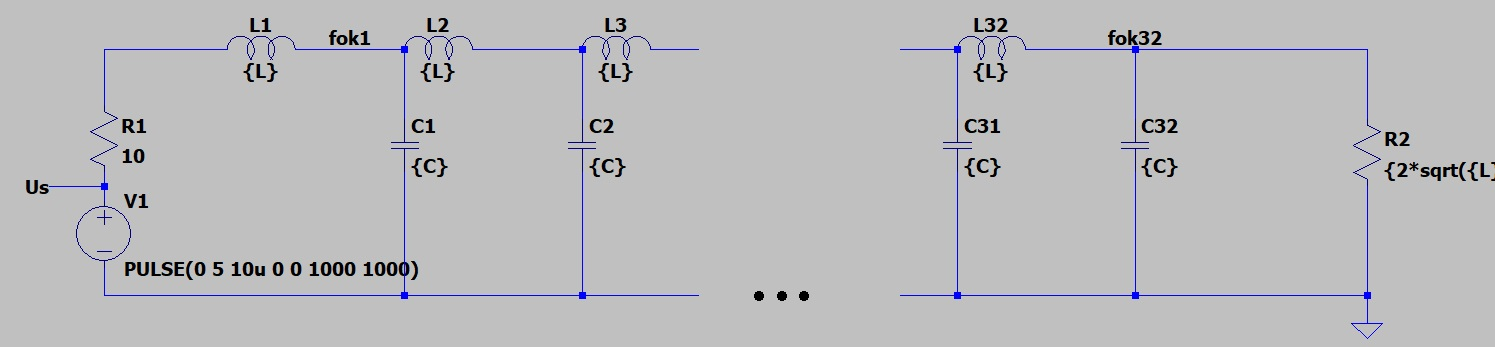
\includegraphics[width=1\textwidth]{figures/ltspicesim.jpg}
    \caption{LTspice szimuláció összeállítása}
    \label{fig:ltspicesim}
\end{figure}

\pagebreak

\begin{figure}[H]
    \centering
    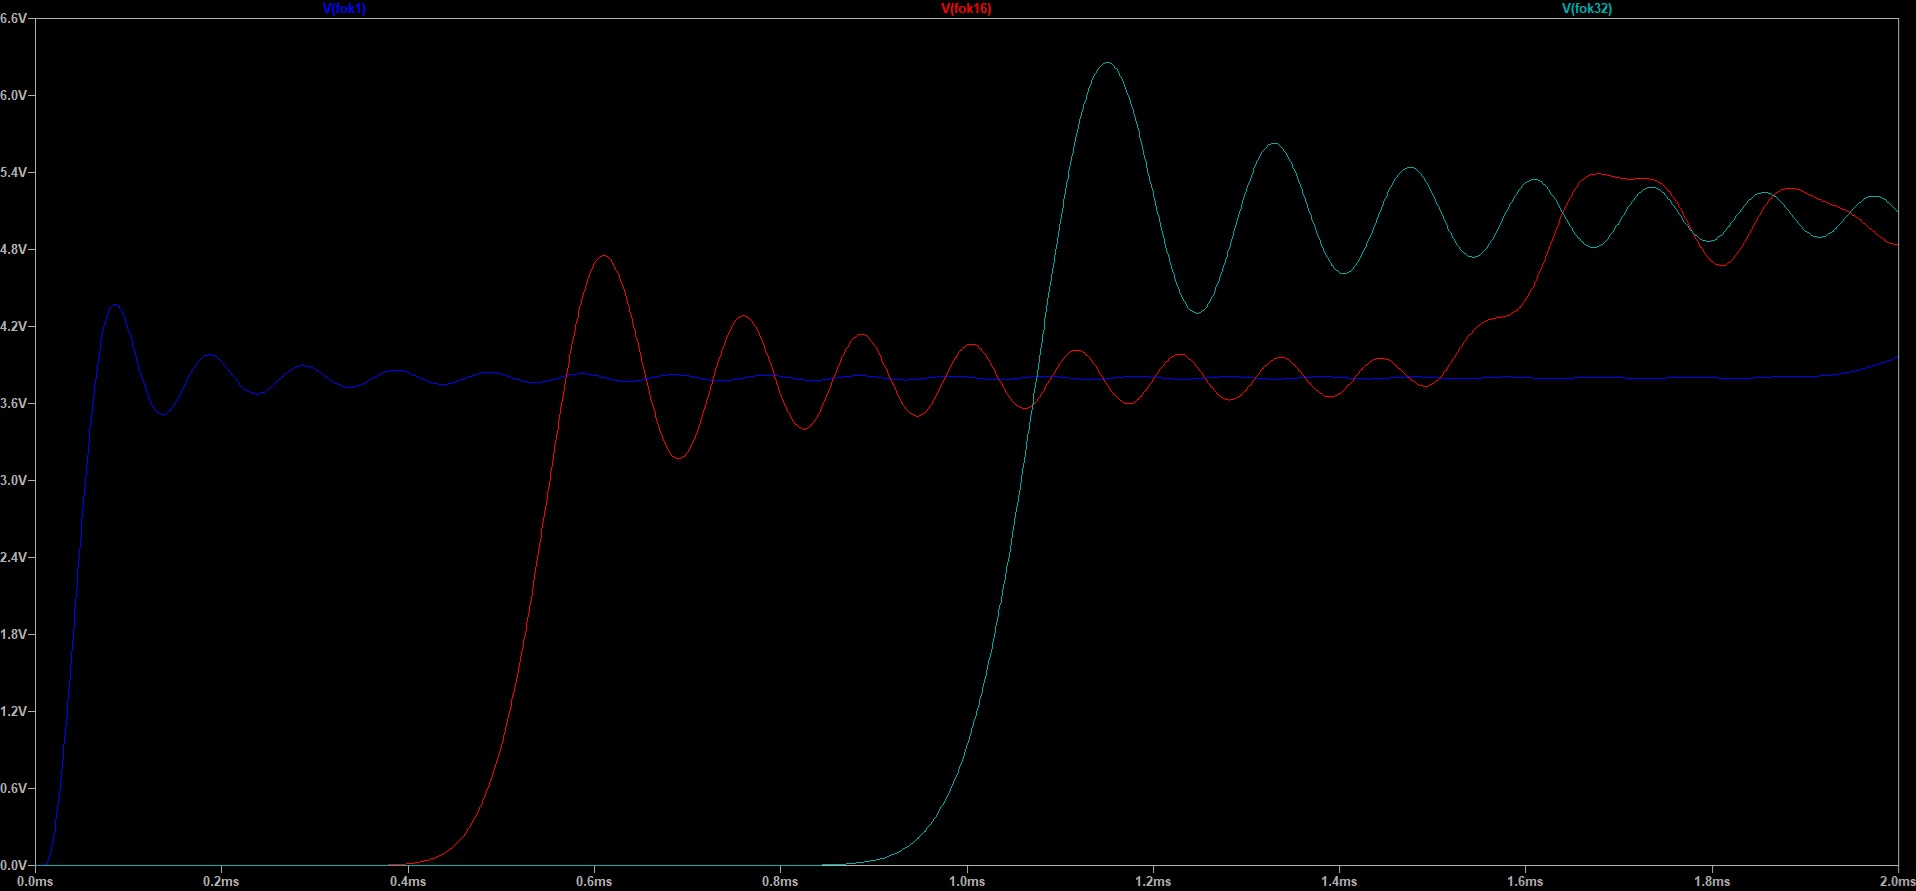
\includegraphics[width=1\textwidth]{figures/32ltspice.jpg}
    \caption{LTspice szimuláció eredménye}
    \label{fig:ltspice}
\end{figure}

\begin{figure}[H]
    \centering
    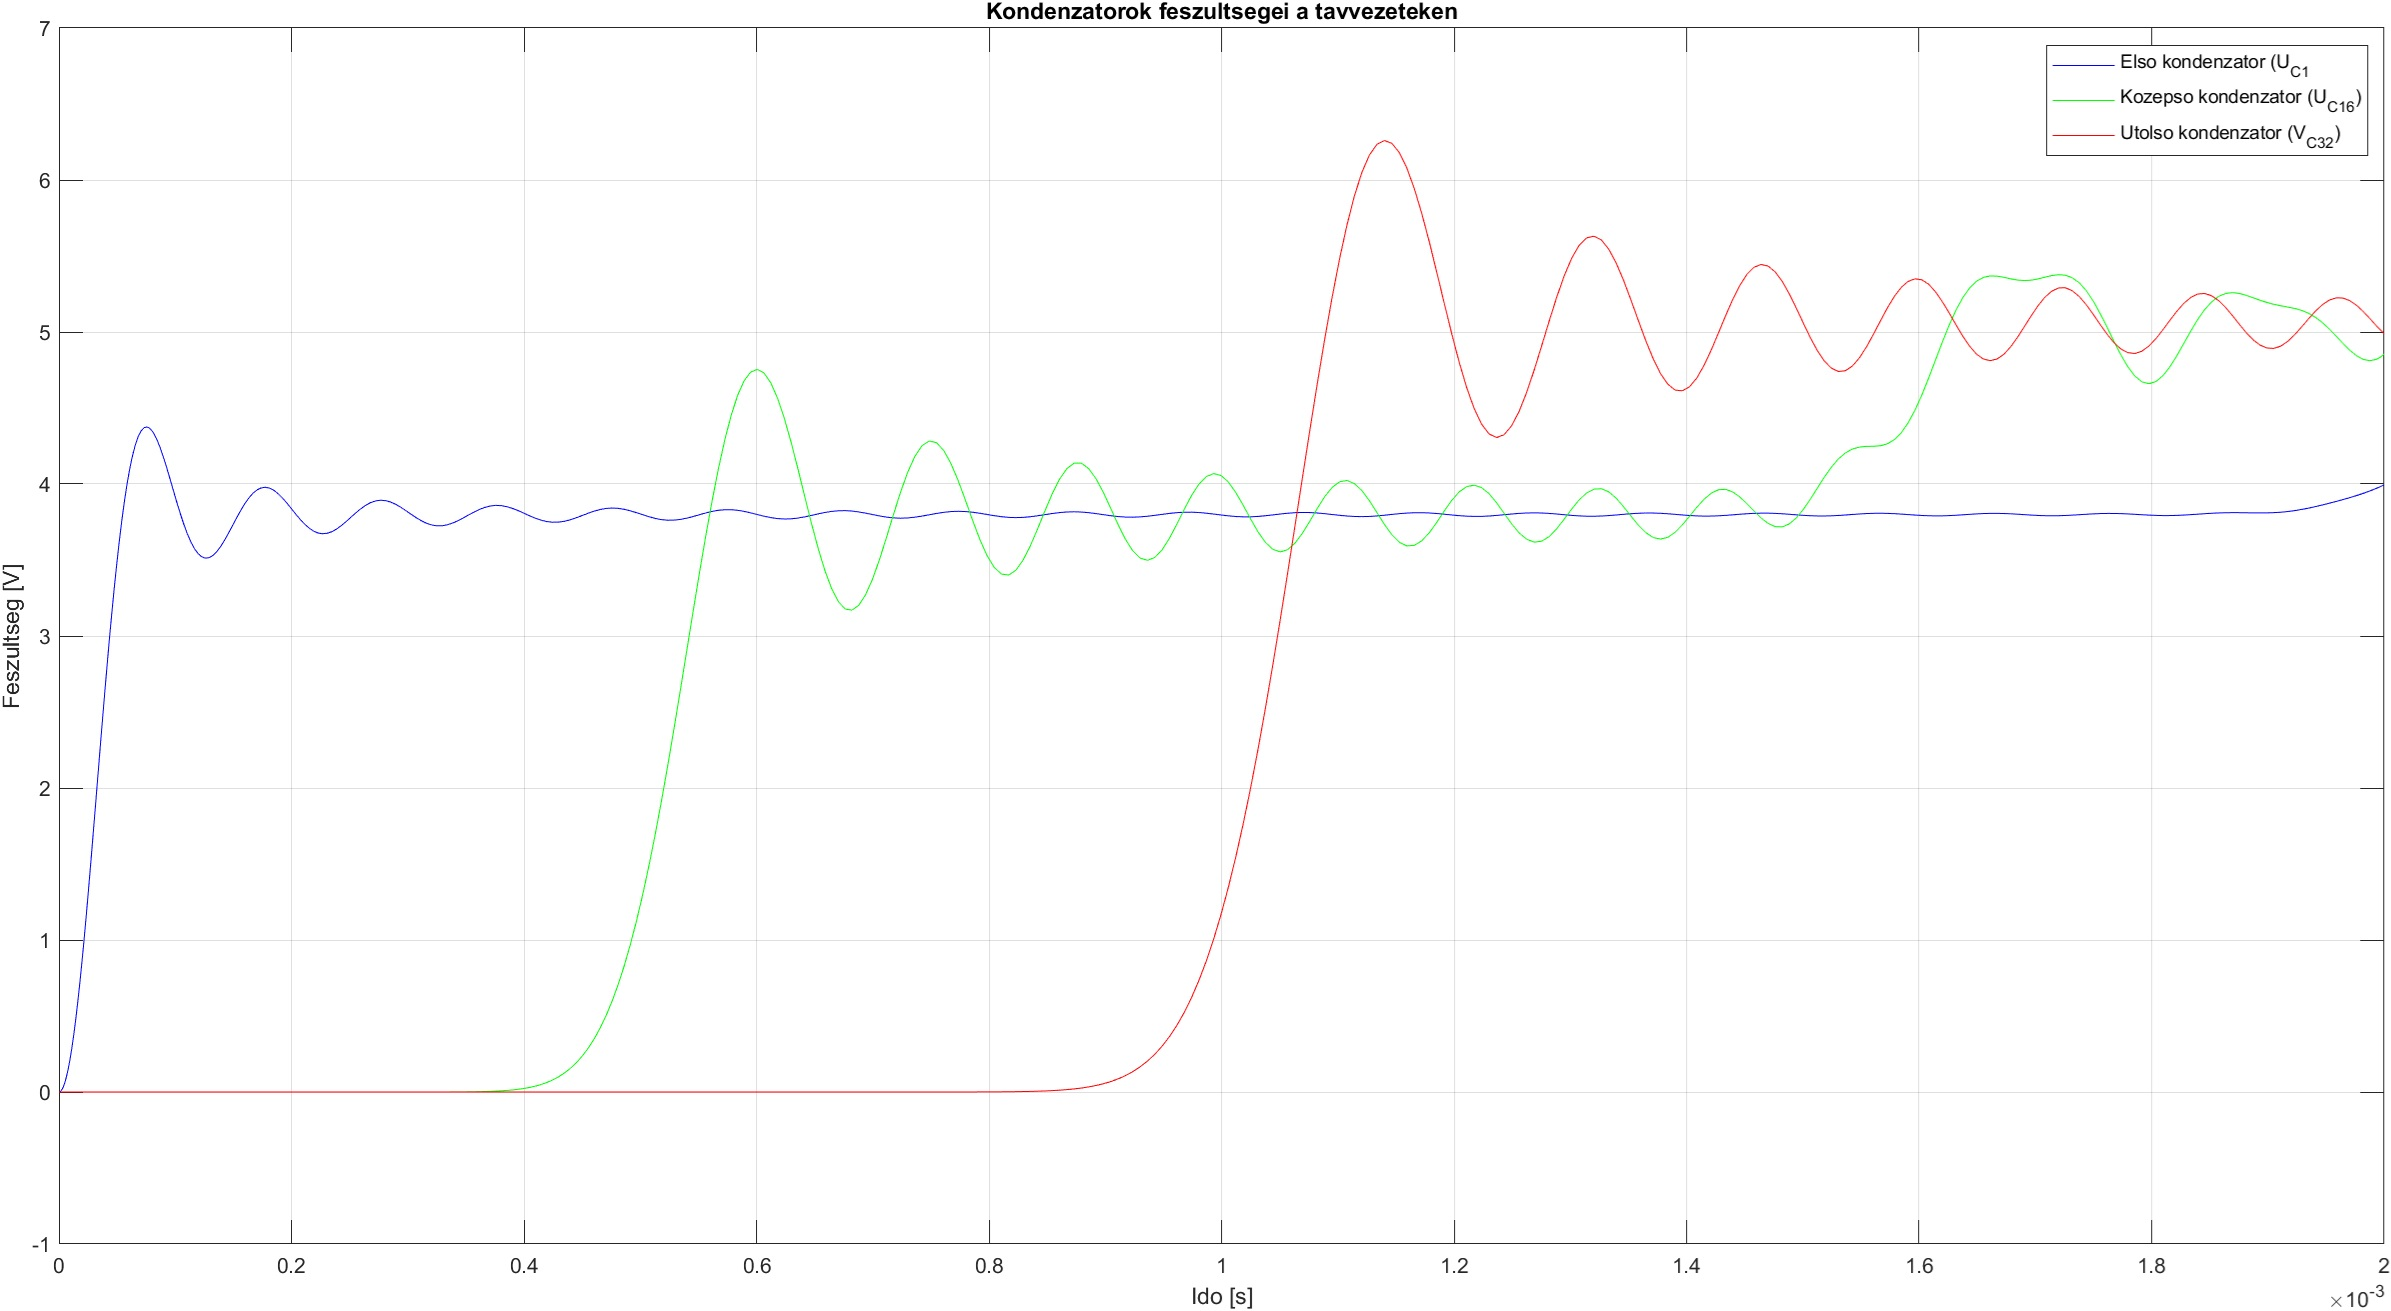
\includegraphics[width=1\textwidth]{figures/32matlab.jpg}
    \caption{MATLAB szimuláció eredménye}
    \label{fig:matlab}
\end{figure}

A szimuláció eredményei alapján következtetéseket vonhatunk le a rendszer stabilitásáról, csillapításáról, a különböző elemek közötti kölcsönhatásokról és a modellezett távvezeték hullámterjedési paramétereiről is.

\pagebreak

\subsection*{Opcionális Ábrázolás}

Lehetőséget biztosítunk a felhasználónak további áramok vagy feszültségek ábrázolására is.

\end{document}